
The current experimental limit on the {\bf neutron EDM} is
$d_n < 3.6 \times 10^{-26}$~e$\cdot$cm at $95\%$ CL~\cite{Chupp:2017rkp},
and for the {\bf electron EDM} $d_e < 1.1 \times 10^{-29}$~e$\cdot$cm at $90\%$
CL~\cite{Andreev:2018ayy}.  
These bounds already test NP at mass scales above $10$ TeV and up to $\sim 10^6$ TeV, see  Fig.~\ref{fig:NPscales} (light yellow columns).  
A variety of other systems 
have also been explored as sensitive probes 
of the EDMs: atoms, protons,  deuterons, muons and different molecules. The current status of the measurements is reported in   Table~\ref{tab:EDM_all}.
The European collaborations lead current neutron EDM searches~\cite{Afach:2015sja}, while the best limits using molecules~\cite{Andreev:2018ayy}, 
diamagnetic atoms~\cite{Graner:2016ses} and 
muons~\cite{Bennett:2008dy} presently come from the experiments conducted in the USA. 

{\setlength{\tabcolsep}{2pt} % Default value: 6pt
\begin{table}
\caption{Current EDM limits. In the table, $Q_m$ denotes the magnetic quadrupole moment, $C_S$ is the scalar form factor, and  $\mu_N$ and $R_{Cs}$ are the nuclear magneton and the nuclear radius of $^{133}C_s$, respectively. For 
further details and a complete review of the experimental 
scenarios see Ref.~\cite{Chupp:2017rkp}. } 
\label{tab:EDM_all} 
{\scriptsize
 \begin{center}
\begin{tabular}{cc}
 \begin{tabular}{lll}
\hline\hline
 & Result & 95\% u.l.\\ \hline 
 \\
& $\quad$ Paramagnetic  systems
 & \\ 
 \hline
 \\
Xe$^m$ & $d_A = (0.7\pm 1.4)\times 10^{-22}$ & $3.1 \times 10^{-22}$ 
e\, cm\\
Cs & $d_A =(-1.8 \pm 6.9) \times 10^{-24}$ &
$1.4 \times 10^{-23}$ 
e\, cm\\ 
& $d_e =(-1.5 \pm 5.7) \times 10^{-26}$& $1.2 \times 10^{-25}$ e\, cm\\ 
& $C_S =(2.5 \pm 9.8) \times 10^{-6}$& $2 \times 10^{-5}$\\
& $Q_m =(3 \pm 13) \times 10^{-8}$& $2.6 \times 10^{-7}$ $\mu_N R_{\rm{Cs}}$\\
Tl &$d_A =(-4.0\pm 4.3) \times 10^{-25}$ & $1.1 \times 10^{-24}$ e\, cm \\
& $d_e =(6.9 \pm 7.4) \times 10^{-28}$& $1.9 \times 10^{-27}$ e\, cm\\
YbF & $d_e =(-2.4 \pm 5.9) \times 10^{-28}$& $1.2 \times 10^{-27}$
e\, cm\\
$^*$ThO & $d_e =(4.3 \pm 3.1 \text{\scriptsize (stat.)}\pm$ \\
& $\pm 2.6 \text{\scriptsize (sys.)}) \times 10^{-30}$& 
$1.1 \times 10^{-29}$ e\, cm\\
{\scriptsize*90\% C.L.}& $C_S$ &$7.1 \times 10^{-10}$ \\
HfF+ & $d_e =(0.9 \pm 7.9) \times 10^{-29}$& 
$1.6 \times 10^{-28}$ 
e\, cm\\
\hline\hline
 \end{tabular}
\hspace*{2mm}&\hspace*{2mm}
\begin{tabular}{lll}
\hline\hline
 & Result & 95\% u.l.\\ \hline 
 \\
& $\quad $ Diamagnetic systems & \\ \hline
\\
$^{199}$Hg & $d_A =(2.2 \pm 3.1) \times 10^{-30}$& 
$7.4 \times 10^{-30}$ 
e\, cm\\
$^{129}$Xe & $d_A =(0.7 \pm 3.3) \times 10^{-27}$& 
$6.6 \times 10^{-27}$ e\, cm\\
$^{225}$Ra & $d_A =(4 \pm 6) \times 10^{-24}$& 
$1.4 \times 10^{-23}$ e\, cm\\
TlF & $d =(-1.7 \pm 2.9) \times 10^{-23}$& 
$6.5 \times 10^{-23}$ e\, cm\\
n& $d_n =(-0.21 \pm 1.82) \times 10^{-26}$&
$3.6 \times 10^{-26}$ e\, cm\\
\hline
\vspace*{1.5mm}\\
&  $\quad $ Particle systems& \\
\hline
\\
$\mu$ & $d_{\mu} =(0.0 \pm 0.9) \times 10^{-19}$&
$1.8 \times 10^{-19}$ e\, cm\\
$\tau$ & $Re(d_{\tau}) =(1.15 \pm 1.70) \times 10^{-17}$&
$3.9 \times 10^{-17}$
e\, cm\\
$\Lambda$ & $d_{\Lambda} =(-3.0 \pm 7.4) \times 10^{-17}$&
$1.6 \times 10^{-16}$
e\, cm\\
& \\
\hline\hline
 \end{tabular}
 \end{tabular}
\end{center}}
\end{table}
}

\setlength{\tabcolsep}{4pt}
\begin{table}
\caption{Summary of the neutron EDM facilities~\cite{PaulESPP19}.}
\label{tab: EDM_status}
\scriptsize
 \begin{center}
 \begin{tabular}{cccc}
\hline\hline
 Place & UCN source & sensitivity $\delta d_n$& start\\ \hline
 ILL &  $^4$He (SuperSANS) at reactor & $10^{-27}$ &2019\\
PIK (Gatchina) & sD$_2$ at PIK reactor  & $2 \times 10^{-28}$ & 2022\\
PSI& sD$_2$ at Spallation Source & $10^{-27}$ &2019\\
TRIUMF &$^4$He at spallation source & $10^{-27}$ &2020\\
SNS (Oak Ridge) &$^4$He at spallation source &
     $2 \times 10^{-28}$ & 2022\\
LANL & sD$_2$ at Spallation Source   &$1-3 \times 10^{-27}$ & 2019\\
RCNP & $^4$He at Spallation Source & $\text{few} \times 10^{-27}$ & under study\\
JPARC & Spallation Source&  $\text{few} \times 10^{-27}$& under study\\
TUM&sD$_2$ at FRMII reactor &$10^{-28}$& $>$ 2022\\
ILL& stack of 100 $^4$He source/EDM cells & $10^{-29}$ &  $>$ 2024\\
ESS& cold neutron beam & $10^{-25}-10^{-26}$ & $>$ 2024\\
    \hline\hline
       \end{tabular}
\end{center}
\end{table}
\setlength{\tabcolsep}{6pt}



In the {\bf short-} and  {\bf mid-term},  several  neutron EDM projects are in  various stages  of  development, as summarized in  Table~\ref{tab: EDM_status}. 
In Europe, they are grouped around reactor facilities (ILL Grenoble, FRM-2 Munich, PNPI Gatchina)  and  intense  proton  spallation  sources  (PSI-Villigen,  ESS-Lund). 
Worldwide, there are three
important neutron EDM projects under development: 
SNS (Oak Ridge), LANL (Los Alamos) and TRIUMF (a  Japanese-Canadian collaboration).




The searches for the EDMs  of  charged  particles  such  as  {\bf protons} or  {\bf deuterons}  can  be  performed using  the  storage  rings \cite{Anastassopoulos:2015ura}. The {\bf short-} and  {\bf mid-term} strategies rely on a step-wise plan. 
The preparatory stages include the exploratory  measurements by the JEDI collaboration
\cite{Jedi_exp} (using COSY at FZJ) to demonstrate the technical feasibility. 
Since 2017, the CPEDM collaboration \cite{Rathmann:2019vtb} has investigated options for the design and construction of a storage ring for  
EDM measurements of charged states. 
The construction of the high-precision
electric-field storage ring could start in 2027, 
and achieve the {\bf proton} EDM sensitivity goal of $10^{-29}$~e$\cdot$cm, at the same level as the neutron EDM sensitivity prospects. 
The prototype ring and the CPEDM stages are host independent.


The ACME Collaboration \cite{Andreev:2018ayy} has recently obtained a new limit on the {\bf electron} EDM, $d_e < 1.1 \times 10^{-29}$~e$\cdot$cm at $90\%$ C.L.~\cite{Andreev:2018ayy}. In the mid-term, 
substantial improvements by a factor of $10-20$ in sensitivity are possible with further developments of the ACME technique, allowing to probe increasingly high scales of new physics. Fig.~\ref{fig:NPscales} illustrates in dark yellow the substantial improvements expected  in the mid-term for the electron and neutron EDMs. 

 So far, the {\bf muon EDM} searches  have been a byproduct of the muon $g-2$ experiments, as presently pursued at FNAL \cite{Chislett:2016jau} and projected at J-PARC \cite{Sato:2017sdn}. In contrast,  PSI intends to exploit their high intensity muon source for a dedicated muon EDM measurement, using a compact storage ring \cite{Crivellin:2018qmi}.   Searches for {\bf molecular and atomic EDMs} are traditionally done in smaller groups at  university laboratories.   In  Europe  this  is,  for  instance,  the  case  for $^{129}$Xe and $^{199}$Hg  atomic EDM searches at TUM (Munich), PTB (Bonn) and FZJ, or the YbF and BaF molecular searches at Imperial College London and University of Groningen, respectively. 
 Some smaller projects  must be hosted at radioactive beam facilities such as ISOLDE. Several EDM experiments also rely on ideal magnetic environments which need advanced shielding  and  often  use  facilities  such as the  magnetically  shielded  room, BMSR-2, at the PTB Berlin or at TUM.


The current EDM upper limits for different fundamental systems and the expected sensitivities at present and planned facilities are summarized in Fig.~\ref{fig:EDM}.


\begin{figure}[t]
\begin{center}
  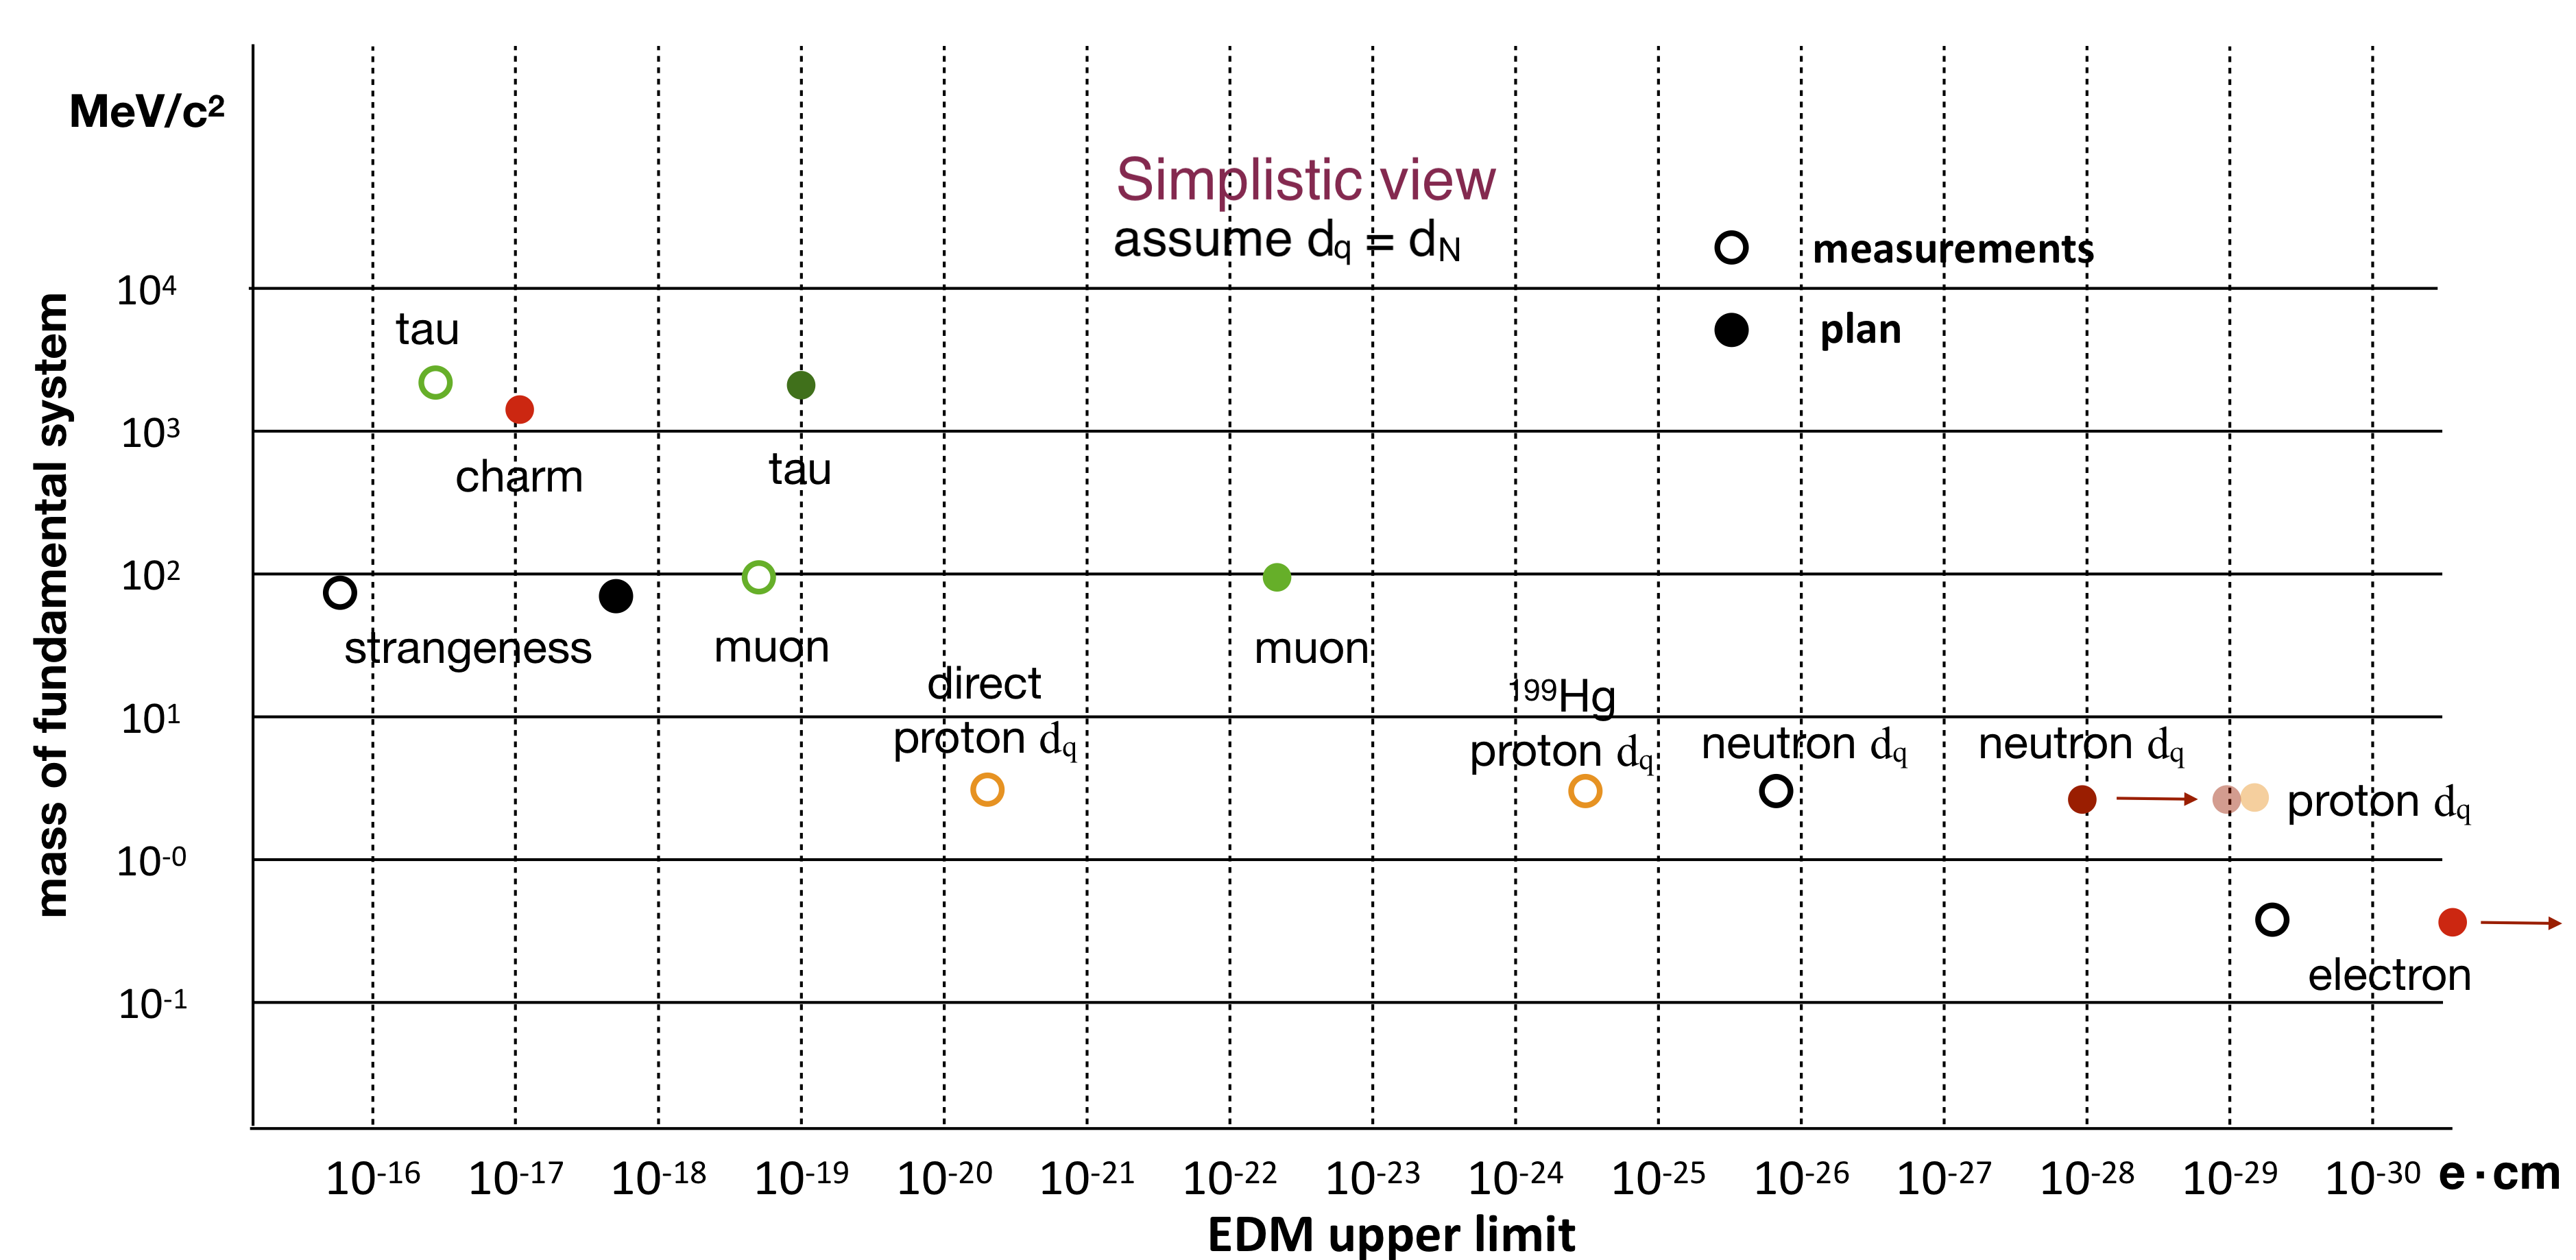
\includegraphics[width=1.0\textwidth]{\main/Flavour/figs/EDM_summary_new}
  \caption{Summary of current EDM limits (empty circles) and short/mid-term  
  planned sensitivities (full circles) for light quarks, strange and charm quarks, electron, muon and tau~\cite{PaulESPP19}.} 
    \label{fig:EDM}
  \end{center}
\end{figure}


Extending EDM searches to heavier probes, such as tau leptons and baryons, can provide qualitatively new BSM probes. These are especially interesting if the structure of the BSM contributions overcomes the inherently lower experimental sensitivities.


For the {\bf tau EDM}, searches could be performed in the {\bf mid-} and {\bf long-term} at Belle~II or, with even  higher sensitivity,  at the Super Charm-Tau (SCT) factories, such as SCT BINP at Novosibirsk~\cite{Bondar:2013cja,Novosibirsk_SCT_input} and STCF/HIEPA in China~\cite{Luo:2018njj,Peng:2018}, 
exploiting the polarized beams and the large statistics of $10^{10} \tau \bar \tau$ pairs per year.


New ideas for {\bf heavy baryon electric and magnetic moment} searches  via spin precession of channeled particles in bent crystals are also being considered. 
These would require extraction of multi-TeV particle beams, which is being studied at
the LHC~\cite{Baryshevsky:2019vou, Mazzolari:2018hsu}. It could also open the door to measurements of magnetic moments of short-lived heavy-quark baryons. 


